%=========================================================================
\sect{Finite-Difference-Method}
\label{Section3}
%=========================================================================

In this chapter we consider the numerical solution of
common and partial differential equations by the 
Finite-Difference-Method. 
There, we compute approximated values of the solution 
at grid points by replacing the derivatives in the 
differential equations with difference quotients. 
This leads to a discrete problem resulting in 
an algebraic system of equations of the form 
$\bA \bx = {\bf f}$. 
The solution $\bx$ are the approximated values of the 
continuous problem at the grid points. 

%-------------------------------------------------------------------------
\ssect{One-dimensional Problem}
\label{Section31}
%-------------------------------------------------------------------------

In this section we want to figure out the way of solving 
ordinary differential equations of 2nd order with the 
Finite-Difference-Method in one-dimensional problems. 
We are looking for a scalar-valued function 
%
\begin{eqnarray}
u: {\cal B} \cup \partial {\cal B} \rightarrow \IR
\end{eqnarray}
%
in the domain ${\cal B} \subset \IR$ with the boundary 
$\partial\cal B$, which satisfies for given 
%
\begin{eqnarray}
f: {\cal B} \rightarrow \IR \and g: \partial {\cal B} \rightarrow \IR
\end{eqnarray}
%
the differential equation in the domain $\cal B$ 
with the boundary conditions 
%
\begin{eqnarray}
\left.
\begin{array}{lclll}
u''(x) & = & - f(x) & \mbox{in} &  {\cal B} \\
    u  & = & g     & \mbox{on} & \partial {\cal B}
\end{array}
\right\} \, . 
\end{eqnarray}
%


\sssect{Discretization 1D}
\label{sec:diskr1d}
%
At first we consider one-dimensional problems, in which 
the considered area ${\cal B} \subset \IR $ 
is defined by 
%
\begin{eqnarray}
{\cal B} := [0,l] \qquad \mbox{with} \qquad l > 0 \, .
\end{eqnarray}
%
For the discretization we choose the constant increment 
$h > 0$ in order to satisfy 
%
\begin{eqnarray}
l = n \cdot h \qquad \mbox{with} \qquad n \in \IN \, . 
\end{eqnarray}

\begin{Figure}[htb]
\begin{center}
\input{\dir/fig303.pstex_t}
\caption{Spatial discretization of the one-dimensional 
problem with constant increment $h$.}
\end{center}
\label{fig300}
\end{Figure}
%
The grid points of the area $\cal B$ are defined by
%
\begin{eqnarray}
{\cal B}_h := \{ ih \mid i = 1, \dots, n -1\} \,.
\end{eqnarray}
%
The points of the boundary $\partial \cal B$ result from
%
\begin{eqnarray}
\partial {\cal B}_h := \{ ih \mid i = 0 \quad \mbox{and} \quad i=n \} \, .
\end{eqnarray}



\sssect{Differential quotients 1D}
First of all we consider the Taylor series expansion of an 
one-dimensional function $u(x+h)$ in the point $x$
%
\begin{equation}
 u(x+h) = u(x) + \frac{1}{1!} u'(x) h 
 + \frac{1}{2!} u''(x) h^2 
 +\frac{1}{3!} u'''(x) h^3 + \dots \, . 
\label{eq:fx+h}
\end{equation}
%
Then the first derivative is computed from solving 
Equation (\ref{eq:fx+h}) with respect to $u'(x)$ 
%
\begin{eqnarray}
\left. 
\begin{array}{l}
u'(x) = \dfrac{u(x+h)-u(x)}{h} 
- \dfrac{1}{2!} u''(x) h - \dfrac{1}{3!} u'''(x) h^2 - \dots \\ [1.1ex]
u'(x) = \dfrac{u(x+h)-u(x)}{h} + O(h)
\end{array} 
\right\} \, .
\label{eq:fstrich1}
\end{eqnarray}
%
Equation $(\ref{eq:fstrich1})_2$ is referred to as
difference quotient. 

\begin{Figure}[htb]
\begin{center}
\input{\dir/fig3_06.pstex_t}
\caption{Visualization of the central difference quotient
(CDQ), the backward difference quotient (BDQ) and the
forward difference quotient (FDQ) of a function $u(x)$.}
\label{fig306}
\end{center}
\end{Figure}%

From the development of $u(x-h)$ at point $x$ we receive
analogously 
%
\begin{equation}
u(x-h) = u(x) - \frac{1}{1!} u'(x) h 
+ \frac{1}{2!} u''(x) h^2 
- \frac{1}{3!} u'''(x) h^3 + \dots \, .
\label{eq:fx-h}
\end{equation}
%
Then, the first derivative yields 
%
\begin{eqnarray}
\left. 
\begin{array}{l}
u'(x) = \dfrac{u(x)-u(x-h)}{h} + \dfrac{1}{2!} u''(x) h 
- \dfrac{1}{3!} u'''(x) h^2 + \dots \\ [1.1ex]
u'(x) = \dfrac{u(x)-u(x-h)}{h} + O(h) 
\end{array} 
\right\} \, ,
\label{eq:fstrich2}
\end{eqnarray}
%
Here, Equation  $(\ref{eq:fstrich2})_2$ is referred to as 
backward difference quotient. 

By summing up Equations (\ref{eq:fstrich1}) and
(\ref{eq:fstrich2}) yields the central difference 
quotient being the approximation of the first derivative 
of $u(x)$ 
%
\begin{eqnarray}
\left. 
\begin{array}{l}
u'(x) = \dfrac{u(x+h)-u(x-h)}{2h}  - \dfrac{1}{3!} u'''(x) h^2 
+ \dots \\ [1.1ex]
u'(x) = \dfrac{u(x+h)-u(x-h)}{2h} + O(h^2)
\end{array} 
\right\} \, .
\end{eqnarray}
%
For the approximaion of the second derivative we sum the
Equations (\ref{eq:fx+h}) and (\ref{eq:fx-h})
%
\begin{eqnarray}
u(x+h)+u(x-h) = 2 u(x) + u''(x) h^2 + O(h^4)
\end{eqnarray}
%
and obtain directly 
%
\begin{eqnarray}
u''(x) = \frac{u(x+h) - 2 u(x) + u(x-h)}{h^2} + O(h^2) \, .
\end{eqnarray}
\begin{table}[htb]
\caption{Differential quotients for an one-dimensional function} 
\[
\fbox{$
\begin{array}{rll} 
\mbox{1.}&\mbox{forward DQ} &u'(x)=\dfrac{u(x+h)-u(x)}{h}\\
 [1.1ex]
\mbox{2.}&\mbox{backward DQ} &u'(x)=\dfrac{u(x)-u(x-h)}{h}\\
 [1.1ex]
\mbox{3.}&\mbox{central DQ} &u'(x)=\dfrac{u(x+h)-u(x-h)}{2h}\\ 
 [1.1ex]
\mbox{4.}&\mbox{2nd derivative}
                   &u''(x)=\dfrac{u(x+h)-2u(x)+u(x-h)}{h^2}\\
\end{array}
$}
\]
\label{table1}
\end{table}

\newpage

{\bf Example:} We consider the function
%
\begin{eqnarray}
u(x) = e^x
\label{eq:ue^x}
\end{eqnarray}
%
and compute the first derivative on the point $x=0$ with the
increment $h=0.1$. 
The approximations yield
%
\begin{eqnarray}
\left.
\begin{array}{lcll}
u'(x=0) & = & 1,05   & \textnormal{forward dq} \\
u'(x=0) & = & 0,95   & \textnormal{backward dq} \\
u'(x=0) & = & 1,0017 & \textnormal{central dq} \\
u'(x=0) & = & 1,0    & \textnormal{exact dq} \\
\end{array}
\right\} \, .
\end{eqnarray}
%
A graphical representation of the function (\ref{eq:ue^x}) 
and its derivative is given in Fig. \ref{diffquo1}.
% 
\begin{Figure}[htb]
\begin{center}
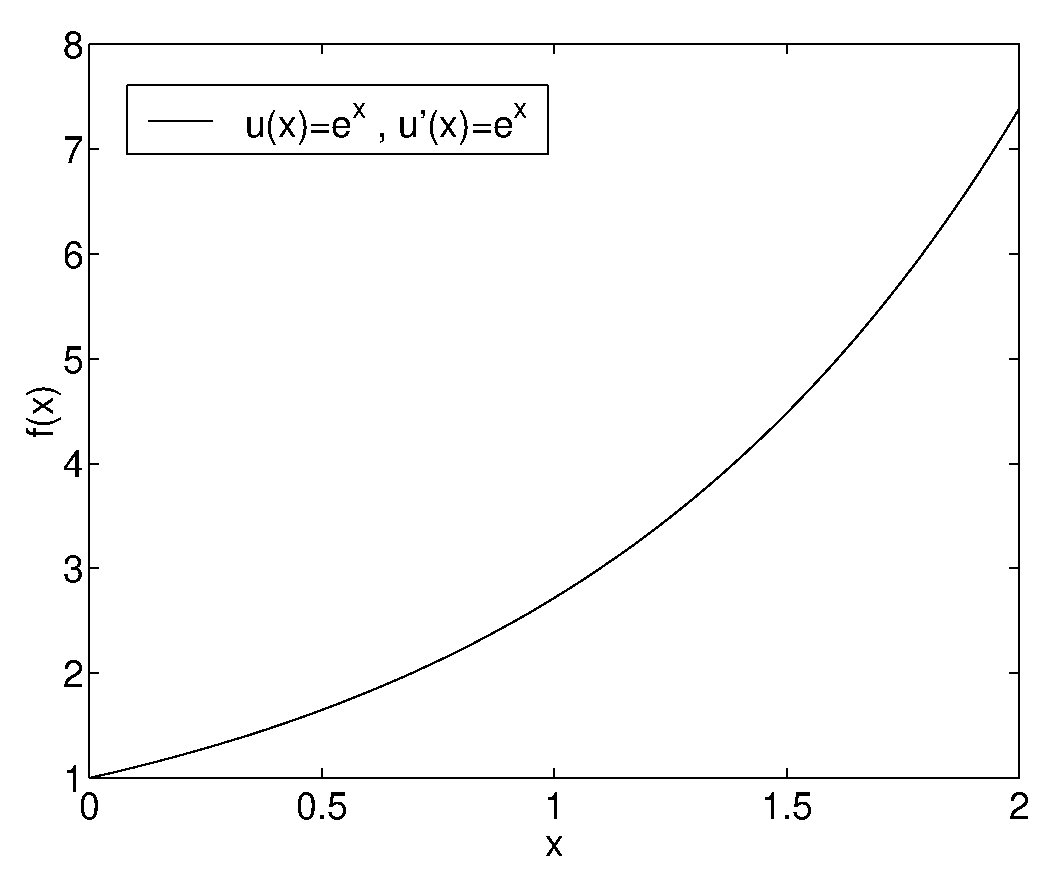
\epsfig{file=\dir/diffquo1d.eps,width=.5\hsize}
\caption{Graphical representation of the function 
$u(x)=e^x$ and its derivative.}
\label{diffquo1}
\end{center}
\end{Figure}
%
















\clearpage
\sssect{Example: Beam with constant cross section.}
%
As a numerical example we consider a beam fixed at 
both sides, loaded by $p(x)$, wich has a constant 
cross-sectional area $A$ and a constant Young's 
modulus $E$, see Fig. \ref{fig302}. 

\begin{Figure}[htb]
\begin{center}
\input{\dir/fig302.pstex_t}
\caption{Model problem: beam with constant stiffness $EA$ 
and distributed loading $p(x)$.} 
\label{fig302}
\end{center}
\end{Figure}%

The model problem is described by an ordinary differential
equation of 2nd order in the domain $\cal B$ and a given
displacement on $\partial \cal B$
%
\begin{eqnarray}
\left.
\begin{array}{rcl}
EA u''(x) & = & - p(x) \\
u(x = 0) & = & 0 \\
u(x = l) & = & 0
\end{array}
\right\} \, .
\label{eq:beisp1}
\end{eqnarray}
%
With $p(x)=p_0 + \Delta \ p \cdot x / l$ and with 
the integration of Equation $(\ref{eq:beisp1})_1$ we get 
the general solution 
%
\begin{equation}
u(x) = - \frac{\Delta p}{6 E A l} x^3 - \frac{p_0}{2 E A} x^2 
       + c_1 x + c_2 \, . 
\end{equation}
%
After incorporating the boundary conditions 
$(\ref{eq:beisp1})_{2,3}$ we obtain 
%
\begin{equation}
u(x) = - \frac{\Delta p}{6 E A l} x^3 - \frac{p_0}{2 E A} x^2 + 
  \left( \frac{p_0 l}{2 E A} + \frac{\Delta p l}{6 E A}  
  \right) x \, .
\label{eq:exaktlou}
\end{equation}
%
In the framework of the Finite-Difference-Method a
discretization of the problem is required.
We consider a discretization with $n+1$ grid points of 
equidistant increments $h$. 
The this leads to the domain discretization 
${\cal B}_h$ as shown in Fig. \ref{fig303}. 

\begin{Figure}[htb]
\begin{center}
\input{\dir/fig303.pstex_t}
\caption{Spatial discretization of the beam.}
\label{fig303}
\end{center}
\end{Figure}
%
We consider the case $p(x)=p_0$ and approximate the 
second derivative by using Table \ref{table1}. 
Then we achieve the approximation 
of the field equations for the individual grid points by 
%
\begin{equation}
 EA \frac{u_{i+1} - 2u_i + u_{i-1}}{h^2} = -p_0 
 \qquad \mbox{for} \qquad i=1,\dots,n-1 \, .
\label{eq:appfe}
\end{equation}
%
The discrete displacements on the boundary are 
%
\begin{equation}
u_0 = 0 \qquad \und \qquad u_{n} = 0 \, .
\label{eq:randbed1}
\end{equation}
%
We write Equation (\ref{eq:appfe}) for every grid point 
and obtain 
%
\begin{eqnarray}
\left.
\begin{array}{rcl}
u_0 - 2 u_1 + u_2 & = & - \dfrac{p_0}{EA} h^2 \\ [1.1ex]
u_1 - 2 u_2 + u_3 & = & - \dfrac{p_0}{EA} h^2 \\ [1.1ex]
\vdots & & \\
u_{n-2} - 2 u_{n-1} + u_{n} & = & - \dfrac{p_0}{EA} h^2 \\
\end{array}
\right\} \, .
\end{eqnarray}
%
Taking into account the boundary 
conditions of Equation (\ref{eq:randbed1}) 
the linear system of equations can be reformulated in 
matrix notation by 
%
\begin{eqnarray}
\left[
\begin{array}{ccccccc}
 2    & -1 & 0  & 0  & 0  & \dots & 0 \\
-1    & 2  & -1 & 0  & 0  & \dots & 0 \\
 0    & -1 & 2  & -1 & 0  & \dots & 0 \\ 
 0    & 0  & -1 & 2  & -1 & \dots & 0\\
\vdots&    &    &    &    &       & \vdots \\
 0    & 0  & 0  & 0  & 0  & \dots & -1\\
 0    & 0  & 0  & 0  & 0  & \dots & 2\\
\end{array}
\right]
\left[
\begin{array}{c}
 u_1    \\  
 u_2    \\ 
 u_3    \\ 
 u_4    \\
 \vdots \\ 
 u_{n-2}\\ 
 u_{n-1}     
\end{array}
\right]
= \frac{h^2}{EA} p_0
\left[
\begin{array}{c}
 1 \\
 1 \\ 
 1 \\
 1 \\    
 \vdots \\ 
 1 \\    
 1 \\
\end{array}
\right]
\end{eqnarray}
%
or in absolute representation
%
\begin{eqnarray}
\bA \cdot \bu = {\bf f} \, .
\end{eqnarray}
%
The solution of the problem with different discretizations
is depicted in Fig. \ref{fig3_04}. 
Specific values of the system and the material are
$l=1$, $A=1$, $p_0=1$, $E=1$.
%

\vspace{1.5cm}
{\bf Exercise:} 
Calculate the displacement $u(x)$ of the beam shown 
in Fig. \ref{fig302} for the loading conditions 
$p_0 = 1$ and $\Delta p = 0$. 
For this purpose consider the discretizations 
$n=2$, $n=4$, $n=11$ and compare the results 
with the exact analytical solution given in 
Equation (\ref{eq:exaktlou}). 

\clearpage
{\bf Solution: }

\setlength{\unitlength}{1cm}
\begin{Figure}[htb]
\begin{picture}(16.0,7.5)
\put(2.3,0.0){\input{\dir/beispiel1.pstex_t}}
\end{picture}
\caption{Displacement u(x) of the beam with constant
cross section for the discretizations $n=2$, $n=4$, $n=11$ 
and the analytical solution.}
\label{fig3_04}
\end{Figure}
%

%
{\small
\begin{verbatim}
      program fdm1d1
c---------------------------------------------------------------------72
c     Beispiel1: Beam with constant stiffness under constant load
c     Numerical solution with the Finite-Difference-Method
c
c     D. Balzani, April 14, 2008
c
c     Parameters:
c...  Input:                                                          
c       n,ll,yo,area,pp
c       n            : Number of grid points
c       ll           : beam length
c       yo           : E-Modulus
c       area         : cross-sectional area
c       pp           : constant load
c...  Output:
c       x            : physical location x
c       u            : displacement u(x)
c...  Local fields:
c       a(nmax,nmax) : coefficient matrix
c       b(nmax)      : right hand side vector
c---------------------------------------------------------------------72
      implicit none
      integer nmax,i,j,n
      parameter (nmax=15)
      real*8 ll,yo,area,pp,hh,fakt
      real*8 a(nmax,nmax),b(nmax),x,u(nmax)
c
c...  Open input and output file
      open (1, file='beispein.dat')
      open (2, file='beispaus.dat')
c
c...  Read system values from file 'beispein.dat'
      read (1, *) n,ll,yo,area,pp 
c 
c...  Initialisize quantities     
      do i=1,n-1
         b(i)=0.d0
	 u(i)=0.d0
	 do j=1,n-1
	    a(i,j)=0.d0
	 end do
      end do
c 
c...  Compute coefficient matrix
      do i=1,n-2
            a(i,i) =  2.d0
	  a(i,i+1) = -1.d0
	  a(i+1,i) = -1.d0
      end do	  
      a(n-1,n-1) = 2.d0
c
c...  Compute right hand side vektor
      hh  = ll/dble(n)
      fakt = (hh*hh*pp)/(yo*area) 
      do i=1,n-1
         b(i) = fakt
      end do
c
c...  Solve linear system of equations
      call gausspivot(a,b,u,nmax,n-1)
c
c...  Plot solution into file 'beispaus.dat'
      write (2,200) 0.d0, 0.d0
      do i=1,n-1
         x = dble(i)*hh
         write (2,200) x, u(i)
      end do
      write (2,200) ll, 0.d0
 200  format (f10.3,f10.3)
      end
\end{verbatim}
}











\newpage  
\sssect{Parabolic problems: equation of heat conduction}

In the previous sections an elliptic differential equation
was considered.
Using the equation of heat conduction as an example we 
now analyze the numerical solution of the parabolic 
differential equation 
%
\begin{equation}
 \vartheta,_t (x,t) = c^2 \vartheta,_{xx} (x,t) 
 \quad \forall \quad x \in {\cal B} \quad \and \quad t > 0
\label{paraw}
\end{equation}
%
in a one-dimensional domain
%
\begin{equation}
 {\cal B} := (0,l) \quad \mbox{with} \quad l>0 \, .
\end{equation}
%
The temperature boundary conditions are
%
\begin{equation}
 \vartheta (0,t) = \vartheta (l,t) = 0 
 \quad \mbox{for} \quad t > 0
\label{eq:rbtemp}
\end{equation}
%
and the initial temperature is given by
%
\begin{equation}
 \vartheta (x,0) = \bar\vartheta (x) 
 \quad \mbox{for} \quad x \in {\cal B} 
 \quad \and \quad t = 0 \, .
\end{equation}
%
The spatial discretization results analogously from
Section \ref{sec:diskr1d}, i.e. with the constant 
increment $h$
%
\begin{equation}
 {\cal B}_h := \{ ih \mid i=1, \dots ,n-1 \} 
 \quad \and \quad \partial {\cal B}_h := \{ ih \mid i=0 
 \quad \and \quad i=n \} \, .
\end{equation}
%
In addition to a spatial discretization a discretization
in time is needed.
Therefore, we choose the grid-increment $\Delta t$ and
get the discrete times $t_j$ by 
% 
\begin{equation}
 t_j = j \Delta t \quad \mbox{for} \quad j=0,1,2, \dots \, . 
\end{equation}
%
We calculate the Taylor polynom in $t$ at a discrete
time $t_j$ according to the results from the 
previous section by using the forward difference 
quotient and obtain 
%
\begin{equation}
 \pp{\vartheta( x_i,t_j)}{t} = 
 \dfrac{\vartheta (x_i,t_j +\Delta t) 
 - \vartheta (x_i,t_j)}{\Delta t} 
 - \frac{\Delta t}{2} \ppp{\vartheta (x_i,\mu_j)}{t^2}
 - \dots \, , 
\label{eq:taypolt}
\end{equation}
%
where $\mu_j \in (t_j , t_{j+1})$ describes the continuous 
time in the discrete time-increment. 
By inserting the approximation for the second derivative 
of $\vartheta$ with respect to $x$ at a point $x_i$ 
yields the difference quotient 
%
\begin{equation}
 \ppp{\vartheta(x_i,t_j)}{x^2} = 
 \dfrac{\vartheta(x_{i+1},t_j) - 2 \vartheta (x_i,t_j) +
 \vartheta(x_{i-1},t_j)}{h^2} - \frac{h^2}{12} 
 \dfrac{\partial^4 \vartheta (\xi_i , t_j)}{\partial x^4} 
 - \dots
\label{eq:taypolx}
\end{equation}
%
with $\xi_i \in (x_{i-1}, x_{i+1})$. 
We disregard the last terms in Equations 
(\ref{eq:taypolt}) and (\ref{eq:taypolx}) and insert 
the difference quotients in (\ref{paraw}) in order 
to obtain the discretized equation 
%
\begin{equation}
 \dfrac{\vartheta(x_i,t_{j+1} ) 
 -\vartheta(x_i,t_j)}{\Delta t}
 -c^2\dfrac{\vartheta(x_{i+1},t_j)
 -2\vartheta(x_i,t_j) + \vartheta (x_{i-1} , t_j)}{h^2} = 0 \, .
\label{eq:diffschema}
\end{equation}
%
In the sequel we denote $\vartheta (x_i , t_j)$ with 
$\vartheta_{ij}$. 
After solving Equation (\ref{eq:diffschema}) 
with respect to $\vartheta_{i,j+1}$ we obtain 
%
\begin{equation}
 \vartheta_{i,j+1} = \left(1-\dfrac{2 c^2 \Delta t}{h^2}\right)
 \vartheta_{ij}+\dfrac{c^2\Delta t}{h^2}(\vartheta_{i+1,j}
 +\vartheta_{i-1,j})
\end{equation}
%
for all $i=1,\dots,(n-1)$ and $j=1,2, \dots $.
For the solution of the discrete problem we proceed as follows;
with given initial temperature $\vartheta(x,0)=\vartheta_1(x)$
the values
%
\begin{equation}
\vartheta_{i0} = \bar\vartheta (x_i) \quad \forall \quad i = 0, 1, \dots , n
\end{equation}
%
are well-known.
Furthermore, with given boundary conditions (\ref{eq:rbtemp})
we obtain
%
\begin{equation}
 \vartheta_{0j} = \vartheta_{nj} = 0
 \quad \forall \quad j = 1, 2, \dots \,.
\end{equation}
%
The abbreviation $\alpha = c^2 \Delta t / h^2$ 
leads to the discretized equation for $j=0$ 
%
\begin{equation}
\vartheta_{i1} = (1 - 2 \alpha ) \vartheta_{i0} + \alpha
(\vartheta_{i+1,0} + \vartheta_{i-1,0}) \, . 
\label{eq:thetai1}
\end{equation}
%
With the unknown temperature vector for the general 
discrete time $t_j$ with $ j = 1, 2 , ...$
%
\begin{equation}
\Bvartheta^{(j)} := [ 
\begin{array}{cccc}
\vartheta_{1j} & \vartheta_{2j} & \dots & \vartheta_{n-1,j}
\end{array}
]^T 
\end{equation}
%
and the given vector of the initial temperature
distribution ($j=0$) 
%
\begin{equation}
\Bvartheta^{(0)} := [ 
\begin{array}{cccc}
\bar\vartheta_1 & \bar\vartheta_2 & \dots & \bar\vartheta_{n-1}
\end{array}
]^T 
\end{equation}
%
the difference scheme (\ref{eq:thetai1}) results for 
time $t_1$ and all positions $x_i$ in the system of 
equations 
%
\begin{equation}
\Bvartheta^{(1)} = \bA \Bvartheta^{(0)} \, .
\label{eq:thetavekt}
\end{equation}
%
Here, $\bA \in \IR^{(n-1) \times (n-1)}$ is a tri-diagonal
matrix of the form
%
\begin{equation}
\bA =  \left[
\begin{array}{ccccc}
(1 - 2 \alpha) &     \alpha     &       0        & \dots  & 0      \\
     \alpha    & (1 - 2 \alpha) &    \alpha      & \dots  & 0      \\
      0        &     \alpha     & (1 - 2 \alpha) & \dots  & 0      \\
    \vdots     &     \vdots     &    \vdots      & \vdots & \vdots \\
       0       &      0         &        0       & \alpha & (1 - 2 \alpha)
\end{array} 
\right] \, .
\end{equation}
%
With Equation (\ref{eq:thetavekt}) we know the 
temperatures at all spatial grid-points at time $t_1$. 
Repeating this process for $j=2$ yields the 
system of equations 
%
\begin{equation}
 \Bvartheta^{(j)} = \bA \Bvartheta^{(j-1)} 
 \quad \with \quad j=2 \, ,
\label{warmex}
\end{equation}
%
which can be computed directly. 
A repeated evaluation of (\ref{warmex}) for $j = 3, 4, ...$
yields the unknown temperature $\Bvartheta^{(j)}$ for all
discrete points $(x_i, t_j)$. 
The temperatures can be computed by the known 
values of the previous time steps. 
This {\it explicit} difference method is referred to as 
forward difference method. 

% \begin{Figure}[htb]
% \begin{center}
% \scalebox{0.85}{\input{\dir/fig3_08.pstex_t}}
% \caption{Visualization of the explicit process.}
% \label{fig3_08}
% \end{center}
% \end{Figure}
%












{\bf Remark:} 
% The forward difference method is 
% only stable, if the spectral radius is
% %
% \begin{equation}
% \rho (\bA^n) \leq 1 \, .
% \label{eq:spektral}
% \end{equation}
% %
% Consider the failure $\be^{(0)}$ determined in the initial 
% spep yields
% % 
% \begin{equation}
% \Bvartheta^{(1)} = \bA (\Bvartheta^{(0)} + \be^{(0)}) \, .
% \end{equation}
% %
% According to this the failure propagates in $\Bvartheta^{(1)}$
% with $\bA \be^{(0)}$.
% In the $j$nd time step the failure is
% %
% \begin{equation}
% \be^{(j)} = \bA^{(j)} \be^{(0)} \, .
% \end{equation}
% %
% The method is only stabil, if the failure is not growing up
% with $j$, i.e. if Equation (\ref{eq:spektral}) holds.
The forward method is only stable, if the condition 
%
\begin{equation}
c^2 \frac{\Delta t}{h^2} \leq \frac{1}{2} \, 
\end{equation}
%
holds. 
Hence, the time increment $\Delta t$ is constrained with 
given increment $h$.
More stable methods are the {\it implicit} difference 
methods. 
Such methods are e.g. obtained by inserting the 
backward difference quotient 
%
\begin{equation}
 \pp{\vartheta(x_i,t_j)}{t} \approx \frac{\vartheta(x_i,t_j ) 
   -\vartheta(x_i,t_{j-1})}{\Delta t} \, .
\label{eq:impfdm}
\end{equation}
%
Introducing Equation (\ref{eq:impfdm}) and 
(\ref{eq:taypolx}) in the differential equation 
yields by disregarding terms of higher order the 
backward difference method 
%
\begin{equation}
 \frac{\vartheta_{ij}-\vartheta_{i,j-1}}{\Delta t}  
 -c^2\frac{\vartheta_{i+1,j}
 -2\vartheta_{ij}+\vartheta_{i-1,j}}{h^2} = 0 \, , 
\end{equation}
for all $i=1,\dots,n-1$ and $j=1,2,\dots$. 
The repeated application of this procedure yields
%
\begin{equation}
\bA \Bvartheta^{(j)} = \Bvartheta^{(j-1)} 
\end{equation}
%
with the tri-diagonal matrix
%
\begin{equation}
\bA = \left[
\begin{array}{ccccc}
(1 + 2 \alpha) &   - \alpha     &       0        & \dots  & 0      \\
   - \alpha    & (1 + 2 \alpha) &  - \alpha      & \dots  & 0      \\
      0        &  -  \alpha     & (1 + 2 \alpha) & \dots  & 0      \\
    \vdots     &     \vdots     &    \vdots      & \vdots & \vdots \\
       0       &      0         &        0       &-\alpha & (1 + 2 \alpha)
\end{array} 
\right] \, .
\end{equation}
%
This is an implicit method (backward difference method) 
since this linear system of equations has to be solved. 

% \begin{Figure}[htb]
% \begin{center}
% \scalebox{0.85}{\input{\dir/fig3_07.pstex_t}}
% \caption{Visualization of the implicit process.}
% \label{fig3_07}
% \end{center}
% \end{Figure}

% {\bf Exercise:} Derive the difference method for the 
% wave equation as an example for a hyperbolic differential
% equation.



















\newpage

%-------------------------------------------------------------------------
\ssect{Two-dimensional problem}
\label{Section32}
%-------------------------------------------------------------------------

In the sequel the Finite-Difference-Method (FDM) is 
considered by means of the Poisson equation 
(elliptic equation) for a two-dimensional, rectangular 
domain $\B$, whose boundary is identified by 
$\partial \B$. 
The precise problem can be reformulated as follows: 

Determine a function 
%
\begin{equation}
u: \B \cup \partial \B \rightarrow \IR
\end{equation} 
%
with given functions
%
\begin{equation}
g: \partial \B \rightarrow \IR 
\quad\mbox{and}\quad  f: \B \rightarrow \IR \, ,
\end{equation}
%
such that
%
\begin{eqnarray}
\left. 
\begin{array}{rcl} 
\Disp-\sum_{i=1}^{d=2}\ppp{u}{x_i^2} &=& f\;\mbox{in}\;\B \\
                                   u &=& g\;\mbox{on}\;\partial\B
\end{array} 
\right\}
\label{eq:fgb}
\end{eqnarray}
%
is fulfilled. 
The unknown function $u(x_1, x_2)$ can be interpreted as 
an electromagnetic potential, displacement of an elastic 
membrane or the planar equilibrium temperature distribution. 
An alternative notation for the right hand side of Equation 
$(\ref{eq:fgb})_1$ is 
%
\begin{equation}
\Delta u = u,_{11} + u,_{22} = 
\sum_{i=1}^2 \ppp{u}{x_i^2}  \, ,
\end{equation}
%
with the Laplace operator $\Delta (\cdot)$.

% If it is asked for a steady state temperature distribution, 
% thus $f = \hat{f} (x,y) = 0$ and we get the Laplace equation
% $\Delta u=0$. 
% The boundary condition $(\ref{eq:fgb})_1$ rules the
% temperature $u(x,y)$ on the boundary $\partial \cal B$ 
% of the domain $\cal B$ and is referred as Dirichlet boundary
% condition.

\sssect{Discretization 2D}

In the framework of the FDM the numerical solution of the 
boundary value problem is computed based on a finite 
number of grid points in $\B\cup\partial\B$.
For this purpose, the derivatives are approximated by 
difference quotients evaluated as discrete function values 
at the grid points. 
From this an algebraic system of equations follows for 
the approximate solution. 
This process is called discretization. 
%
\begin{Figure}[htb]
\unitlength1cm
\begin{picture}(16.0, 5.5)
\put(-0.6,-0.5){\input{\dir/fig3_01.pstex_t}}
\end{picture}
\setlength{\baselineskip}{11pt}
\caption{Discretization of the domain 
${\cal B}=(0,l_x)\times(0,l_y)$ yields the 
discretized domain ${\cal B}_h$ with 
$(n_x + 1) \cdot (n_y+1)$ grid points.} 
\label{fig3_01}
\end{Figure}
%

Here, we consider a two-dimensional problem $(d=2)$ and
choose for the discretization the increments $h_x , h_y > 0$ 
in both directions. 
In Fig. \ref{fig3_01} a rectangular domain
%
\begin{equation}
 \B := (0, l_x) \times (0,l_y) 
 \qquad\mbox{with} \quad l_x , l_y > 0
\end{equation}
%
is illustrated.
For simplification an equidistant increment $h_x$ is 
chosen in $x$-direction and $h_y$ in $y$-direction, 
respectively, i.e.
% 
\begin{equation}
l_x = n_x h_x 
\qquad \mbox{and} \qquad 
l_y = n_y h_y 
\qquad \mbox{with} \qquad 
n_x , n_y \in \IN \, .
\end{equation}
%
The grid points in the domain $\B$ are defined by
%
\begin{equation}
 \B_h := \{(ih_x,jh_y)\mid i=1,\dots,n_x-1;j=1,\dots,n_y-1\}
\end{equation}
%
and the grid points on the boundary $\partial \B$ by
%
\begin{equation}
\partial \B_h 
 := \{ (ih_x,jh_y)\mid i\in\{0,n_x\},j \in \{0,\dots,n_y\}\;
 \mbox{or} \; i \in \{0,\dots,n_x\},j \in\{0, n_y\}\} \,.
\end{equation}
%
% All of the grid points results from 
% ${\cal B}_h \bigcup \partial {\cal B}_h$.
Please note that here we focus on a boundary value 
problem which is rate-independent, thus, here no 
time discretization is required. 



\sssect{Difference quotients 2D}
The approximation formula for each point in the 
domain ${\cal B}_h$ is computed by 
%
\begin{equation}
\ppp{u(x_i,y_j)}{x^2} = \frac{u(x_{i+1},y_j) - 2 u(x_i,y_j) + 
u(x_{i-1},y_j)}{h_x^2} - \frac{h_x^2}{12} 
\frac{\partial^4 u(\xi_i,y_j)}{\partial x^4} - \dots
\label{eq:dudx}
\end{equation}
%
for $\xi_i \in [x_{i-1}, x_{i+1}]$. 
With the Taylor polynom for $y$ at a point $y_j$ we get 
analogously 
%
\begin{equation}
 \ppp{u(x_i,y_j)}{y^2} = \frac{u(x_{i},y_{j+1}) 
 - 2 u(x_i,y_j) + u(x_i,y_{j-1})}{h_y^2} 
 -\frac{h_y^2}{12}\frac{\partial^4 u(x_i,\eta_j)}{\partial y^4}
 -\dots
\label{eq:dudy}
\end{equation}
%
for $\eta_j \in [y_{j-1}, y_{j+1}]$. 
Inserting Equation (\ref{eq:dudx}) and (\ref{eq:dudy}) 
in the Poisson equation yields 
%
\begin{eqnarray}
\left.
\begin{array}{l}
\dfrac{u(x_{i+1},y_j) - 2 u(x_i,y_j) + u(x_{i-1},y_j)}{h_x^2} \\
+ \dfrac{u(x_{i},y_{j+1}) - 2 u(x_i,y_j) + u(x_i,y_{j-1})}{h_y^2} \\
= f(x_i,y_j) + \dfrac{h_x^2}{12} \dfrac{\partial^4 u(\xi_i,y_j)}{x^4} +  
\dfrac{h_y^2}{12} \dfrac{\partial^4 u(x_i,\eta_j)}{y^4} 
\end{array}
\right\} 
\begin{array}{lcl}
\forall & i=1,2,\dots,(n_x-1) & \and \\ & j=1,2,\dots,(n_y-1). & 
\end{array}
\end{eqnarray}
%
We set the boundary conditions 
%
\begin{equation}
 u(x_i,y_0) = g(x_i,y_0) 
 \quad\and\quad u(x_i,y_m) = g(x_i,y_m)
 \quad\forall \, i=1,2,\dots,(n_x-1) 
\end{equation}
and
\begin{equation}
 u(x_0,y_j) = g(x_0,y_j) \quad\and\quad u(x_n,y_j)=g(x_n,y_j) 
 \quad\forall \, j=0,1,\dots,n_y.
\end{equation}

Let us denote the approximation of $u(x_i,y_j)$ as $u_{ij}$,
then a straighforward transformation leads to the 
discrete form 
% of the order $O(h_x^2 + h_y^2)$ is
%
\begin{eqnarray}
\left.
\begin{array}{c}
2 \left[ \left( \dfrac{h_x}{h_y} \right)^2 + 1 \right] 
u_{ij} - (u_{i+1,j} +
u_{i-1,j}) - \left( \dfrac{h_x}{h_y} \right)^2 (u_{i,j+1} + u_{i,j-1}) = 
- h_x^2 f(x_i,y_j) \\ \bigskip 
\forall \quad i=1,2,\dots,(n_x-1) \quad \and \quad
j=1,2,\dots,(n_y-1) \\ 
u_{0j} = g(x_0,y_j) \, , \, u_{nj} = g(x_n,y_j)  \, , \,
u_{i0} = g(x_i,y_0) \, , \, u_{im} = g(x_i,y_m) \\ [1.2ex]
\forall \quad i=1,2,\dots,(n_x-1) \, ; \quad
j=1,2,\dots,(n_y-1) \\
\end{array}
\right\} \, .
\label{eq:fdmappr}
\end{eqnarray}
%
For $h_x = h_y = h$ we get the standard five-point stencil 
%
\begin{eqnarray}
\frac{1}{h^2}
\left[
\begin{array}{rrr}
0 & -1 & 0 \\
-1 & 4 & -1 \\
0 & -1 & 0 
\end{array}
\right] \, .
\end{eqnarray}
%
{\bf Example:} Computation of the stationary temperature 
distribution in a slim, quadratic metal plate with a 
length of $l_x=l_y=l=0,5$ m. 
The given boundary temperatures are illustrated in Fig.
\ref{fig308}.

\begin{Figure}[htb]
\begin{center}
\unitlength1cm
\input{\dir/fig308.pstex_t}
\setlength{\baselineskip}{11pt}
\caption{Quadratic plate with given boundary temperature.}
\label{fig308}
\end{center}
\end{Figure}%

The physical problem is described by the mathematical 
formulation 
%
\begin{eqnarray}
\ppp{\vartheta}{x^2}(x,y) + \ppp{\vartheta}{y^2}(x,y) = 0 \quad 
\forall \quad (x,y) \in \cal B \, , 
\end{eqnarray}
%
which is referred to as Laplace equation. 
The domain $\cal B$ is defined by
%
\begin{eqnarray}
{\cal B} := \{ (x,y) | 0<x<0.5 \, , \, 0<y<0.5 \} 
\end{eqnarray}
%
and the boundary temperatures are
%
\begin{eqnarray}
\vartheta(0,y)=0 \, , \, \vartheta(x,0)=0 \, , \, 
\vartheta(x,0,5)=200 x \, , \, \vartheta(0,5,y)=200 y \, . 
\end{eqnarray}

In this example we are interested in the solution of 
the boundary value problem for the number of grid 
points given by $n_x=n_y=4$, see 
Fig. \ref{fig307}. 

\begin{Figure}[htb]
\begin{center}
\unitlength1cm
\input{\dir/fig307.pstex_t}
\setlength{\baselineskip}{11pt}
\caption{Discretization of the metal plate with 9 grid points 
in the domain and 16 boundary points.}
\label{fig307}
\end{center}
\end{Figure}%

Compare the numerical results with the exact analytical 
solution 
%
\begin{eqnarray}
\vartheta(x,y) = 400 xy \, .
\end{eqnarray}
%

At the boundary nodes the temperature is known, whereas 
the temperature at the internal grid points has to be 
computed. 
These remaining 9 grid points are numbered according 
to Fig. \ref{fig307}. 

Regarding equation $(\ref{eq:fdmappr})_1$  we get for 
$h_x = h_y = h$ with $\vartheta \equiv u$ the expression
%
\begin{equation}
4 \vartheta_{i,j} - ( \vartheta_{i+1,j} + \vartheta_{i-1,j}) - 
( \vartheta_{i,j+1} + \vartheta_{i,j-1} ) = - h^2 f(x_i,y_j) \, .
\label{eq:fdmtemp}
\end{equation}
%
Utilizing the Equation (\ref{eq:fdmtemp}) for point 7
with $i=1$ and $j=1$ yields
%
\begin{equation}
4 \vartheta_{1,1} - ( \vartheta_{2,1} + \vartheta_{0,1}) - 
( \vartheta_{1,2} + \vartheta_{1,0} ) = 0 \, .
\end{equation}
%
For simplification we use the transformation 
$\vartheta_{1,1} =: \vartheta_{7}, 
\vartheta_{1,2} =: \vartheta_{12}, 
\vartheta_{2,1} =: \vartheta_{8}$ and obtain 
%
\begin{equation}
 4\vartheta_7 - (\vartheta_8+0)-(\vartheta_{12}+0 ) = 0 \,,
\end{equation}
%
respectively.
The system of equations, which has to be solved, is given
by application of the difference sheme for all inner
grid points
%
\begin{eqnarray}
\left[ 
\begin{array}{rrrrrrrrr}
 4 & -1 &  0 & -1 &  0 &  0  &  0 &  0 &  0 \\
-1 &  4 & -1 &  0 & -1 &  0  &  0 &  0 &  0 \\
 0 & -1 &  4 &  0 &  0 & -1  &  0 &  0 &  0 \\
-1 &  0 &  0 &  4 & -1 &  0  & -1 &  0 &  0 \\
 0 & -1 &  0 & -1 &  4 & -1  &  0 & -1 &  0 \\
 0 &  0 & -1 &  0 & -1 &  4  &  0 &  0 & -1 \\
 0 &  0 &  0 & -1 &  0 &  0  &  4 & -1 &  0 \\
 0 &  0 &  0 &  0 & -1 &  0  & -1 &  4 & -1 \\
 0 &  0 &  0 &  0 &  0 & -1  & 0  & -1 &  4 \\
\end{array}
\right] 
\left[ 
\begin{array}{c}
\vartheta_7 \\ \vartheta_8 \\ \vartheta_9 \\ \vartheta_{12}\\ 
\vartheta_{13} \\
\vartheta_{14} \\ \vartheta_{17} \\ \vartheta_{18} \\ \vartheta_{19}
\end{array}
\right] = 
\left[ 
\begin{array}{r}
0 \\ 0 \\ 25 \\ 0 \\ 0 \\ 50 \\ 25 \\ 50 \\ 150
\end{array}
\right] \, . 
\end{eqnarray}
%
The solution of this system of equations is 
%
\begin{eqnarray*}
\Bvartheta = \left[ 
\begin{array}{r}
6,25 \\ 12,5 \\ 18,75 \\ 12,5 \\ 25,0 \\ 37,5 \\ 18,75 \\ 37,5 \\ 56,25 
\end{array}
\right]
\end{eqnarray*}
%
% Due to the fact that in this example the solution variable 
% (temperature) is distributed linearly, the numerical 
% solution is exact, since inserting a difference quotient 
% as the approximation represents a linear interpolation 
% between the grid point quantities. 


%
{\small
\begin{verbatim}
      program fdm
c---------------------------------------------------------------------72
c     Example 2: Metal plate with stationary temperature distribution
c     Numerical solution with Finite-Difference-Method
c
c     D. Balzani, April 21, 2008
c
c     Parameters:
c     n        size of coefficient matrix a
c     a(n,n)   coefficient matrix
c     b(n)     right hand side vector
c...  output
c     x(n)     solution vector
c----------------------------------------------------------------------
      implicit none
c
      integer n,nmax,i,k,j
      parameter (nmax=10)                                            
      real*8 a(nmax,nmax),b(nmax),x(nmax)
c
c...  Number of inner grid points
      n = 9
c
c...  Open output file
      open (1, file='example2.dat')
c
c...  Initialize fields
      do i=1,n
        do j=1,n
          a(i,j) = 0.d0
        enddo
        b(i) = 0.d0
      enddo
c
c...  coefficient matrix a
      do i=1,n
        a(i,i) = 4.d0
      enddo
      a(1,2) = -1.d0
      a(1,4) = -1.d0
      a(2,3) = -1.d0
      a(2,5) = -1.d0
      a(3,6) = -1.d0
      a(4,5) = -1.d0
      a(4,7) = -1.d0
      a(5,6) = -1.d0
      a(5,8) = -1.d0
      a(6,9) = -1.d0
      a(7,8) = -1.d0
      a(8,9) = -1.d0
c     symmetrize
      do i=1,n
        do j=i+1,n
          a(j,i) = a(i,j)
        enddo
      enddo
c
c...  right hand side vector
      b(3) = 25.d0
      b(6) = 50.d0
      b(7) = 25.d0
      b(8) = 50.d0
      b(9) = 150.d0
c
c...  screen output
      write(*,*)
      write(*,*)'coefficient matrix:'
      do i=1,n
        write(*,100)(a(i,j),j=1,n)
      enddo
      write(*,*)
      write(*,*)'right hand side:'
      do i=1,n
        write(*,200)b(i)
      enddo
      write(*,*)
c
c...  solve system of equations
      call gausspivot(a,b,x,nmax,n)
c
c...  screen output of solution vector
      write(*,*)'solution vector:'
      do i=1,n
        write(*,200)x(i)
      enddo
      write(*,*)
c
c...  file output of solution vector
      do i=1,n
        write (1, 200) x(i)
      end do	
c
 100  format (9f6.1)
 200  format (f10.3)
      end 
\end{verbatim}
}
%




%%% Local Variables: 
%%% mode: plain-tex
%%% TeX-master: t
%%% End: 
